\chapter{Creating a test suite: the "tests" folder}
\label{chap:creating_a_test_suite}

\section{Methodology}

Writing a Parsing Expression Grammar (see next part of the thesis) requires constant vigilance in order to make sure
that any rule change doesn't impact several nodes of the grammar at the same time, thus breaking its tree. Running test
sentences one by one, by hand, would be time consuming and not very scientific (especially if there are hundreds of test sentences).
Thus, a test suite must be created in order to evaluate the validity and degree of completeness of the PEG.
Additionally, a data set with enough sentences to parse is required. Thankfully, throughout the chapters of \citetitle{cowan1997complete},
\citeauthor{cowan1997complete} gives us a trove of example sentences.\newline

Using the PyTest Python library \footcite{pytest8.3.2}, a test suite will be constructed in order to run the parser on
all sentences collected.

\section{Breakdown of the folder}

The code produced is found at Annex \ref{appendix:parser-testing-annex}.

\subsection*{conftest.py file}

\subsection*{test\_gentufa.py file}

\subsection*{sentences directory}

The "sentences" directory contains many files, one per chapter, listing the sentences which will compose the dataset.

\newpage

\section{Examples of usage}

The test suite is run by executing a makefile at the root of the code directory with the following command: \textbf{make tests}\newline

Once executed, all tests will run and display a test run summary. There are two possible outcomes: either all tests pass correctly,
or errors have been introduced. Thankfully, due to proper error-handling and test cases management, the test suite outputs all errors,
what part of the grammar is affected, what sentences the errors correspond to,
and which chapter of the book the sentence hails from. This is extremely useful in order to debug at
which layer of the grammar the error was introduced. The following figures display examples of these two possible outcomes:\newline

\begin{figure}[H]
\hspace{-1.1cm}
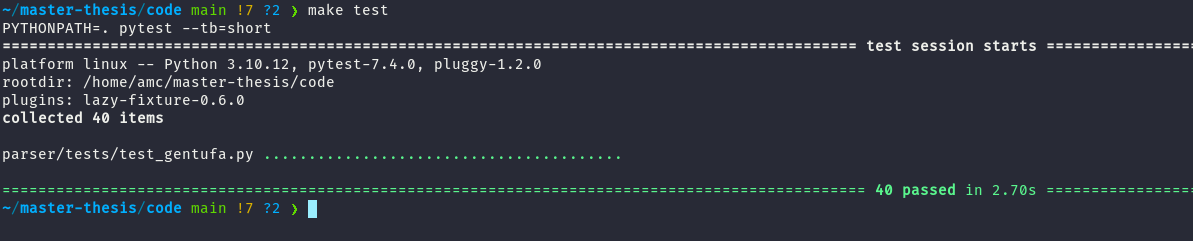
\includegraphics[scale=0.43]{images/pytest_output_pass.png}
\caption{Pytest Output Example - All tests passing}
\end{figure}

\begin{figure}[H]
\hspace{-2.2cm}
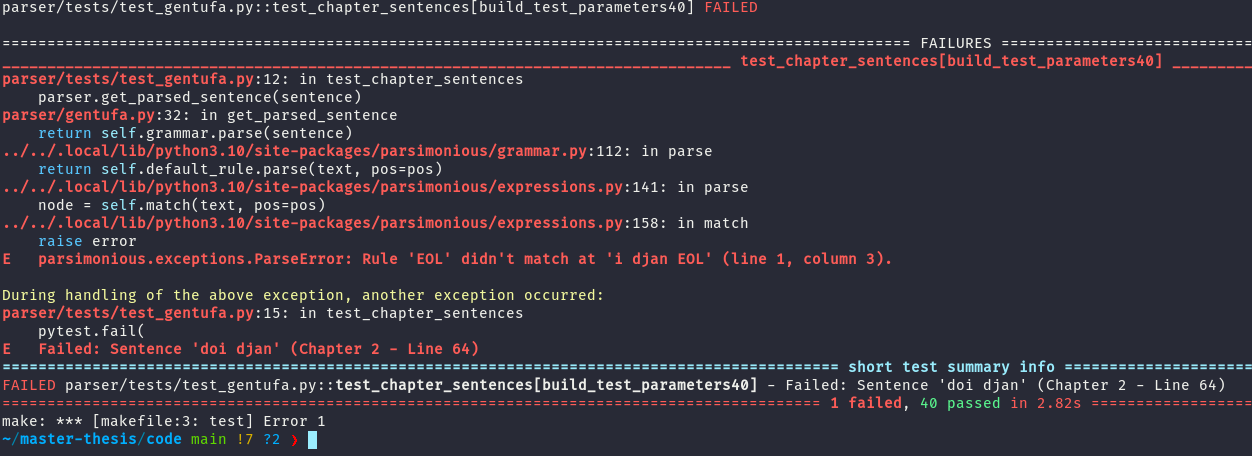
\includegraphics[scale=0.43]{images/pytest_output_fail.png}
\caption{Pytest Output Example - An error occured}
\end{figure}